\documentclass[a4paper,11pt,oneside]{article}

\usepackage[utf8]{inputenc}
\usepackage[a4paper,top=3cm,bottom=3cm,left=3cm,right=3cm]{geometry}
\renewcommand{\familydefault}{\sfdefault}
\usepackage{helvet}
\usepackage[english]{babel}     %% typographie française
\usepackage[style=numeric,language=english, sorting=none]{biblatex}
\usepackage{parskip}		%% blank lines between paragraphs, no indent
\usepackage[margin=1cm]{caption}%% give long captions a margin
\usepackage{booktabs}           %% typesetting nice tables
\usepackage[pdftex]{graphicx}	%% include graphics, preferably pdf
\graphicspath{ {./images/} }
\usepackage[pdftex]{hyperref}	%% many PDF options can be set here
\pdfadjustspacing=1		%% force LaTeX-like character spacing

\newcommand{\myname}{Tianyao Chen}
\newcommand{\mytitle}{Deep Learning for Detecting Amphoras in Ancient Shipwrecks}
\newcommand{\mysupervisor}{Prof. Dr. Andreas Birk}

\hypersetup{
  pdfauthor = {\myname},
  pdftitle = {\mytitle},
  pdfkeywords = {},
  colorlinks = {true},
  linkcolor = {blue}
}

\addbibresource{Tianyao_Chen_bachelor_thesis.bib}

\begin{document}
  \pagenumbering{roman}

  \thispagestyle{empty}

  \begin{flushright}
    
\includegraphics[scale=0.8]{bsc-logo}
  \end{flushright}
  \vspace*{40mm}
  \begin{center}
    \huge
    \textbf{\mytitle}
  \end{center}
  \vspace*{4mm}
  \begin{center}
   \Large by
  \end{center}
  \vspace*{4mm}
  \begin{center}
    \LARGE
    \textbf{\myname}
  \end{center}
  \vspace*{20mm}
  \begin{center}
    \Large
    Bachelor Thesis in Computer Science
  \end{center}
  \vfill
  \begin{flushleft}
    \large
    Submission: \today \hfill Supervisor: \mysupervisor \\
    \rule{\textwidth}{1pt}
  \end{flushleft}
  \begin{center}
    Jacobs University Bremen $|$ Department of Computer Science and Electrical Engineering
  \end{center}

  \newpage
  \thispagestyle{empty}

  \subsection*{English: Declaration of Authorship}

  I hereby declare that the thesis submitted was created and written
  solely by myself without any external support. Any sources, direct
  or indirect, are marked as such. I am aware of the fact that the
  contents of the thesis in digital form may be revised with regard to
  usage of unauthorized aid as well as whether the whole or parts of
  it may be identified as plagiarism. I do agree my work to be entered
  into a database for it to be compared with existing sources, where
  it will remain in order to enable further comparisons with future
  theses. This does not grant any rights of reproduction and usage,
  however.

  This document was neither presented to any other examination board
  nor has it been published.

  \subsection*{German: Erklärung der Autorenschaft (Urheberschaft)}

  Ich erkläre hiermit, dass die vorliegende Arbeit ohne fremde Hilfe
  ausschließlich von mir erstellt und geschrieben worden ist. Jedwede
  verwendeten Quellen, direkter oder indirekter Art, sind als solche
  kenntlich gemacht worden. Mir ist die Tatsache bewusst, dass der
  Inhalt der Thesis in digitaler Form geprüft werden kann im Hinblick
  darauf, ob es sich ganz oder in Teilen um ein Plagiat handelt. Ich
  bin damit einverstanden, dass meine Arbeit in einer Datenbank
  eingegeben werden kann, um mit bereits bestehenden Quellen
  verglichen zu werden und dort auch verbleibt, um mit zukünftigen
  Arbeiten verglichen werden zu können. Dies berechtigt jedoch nicht
  zur Verwendung oder Vervielfältigung.

  Diese Arbeit wurde noch keiner anderen Prüfungsbehörde vorgelegt
  noch wurde sie bisher veröffentlicht.

  \vspace{20mm}

  Date, Signature

  \newpage

  \section*{Abstract}

  Consider this a separate document, although it is submitted together
  with the rest. The abstract aims at another audience than the rest
  of the proposal. It is directed at the final decision maker or
  generalist, who typically is not an expert at all in your field, but
  more a manager kind of person. Thus, don't go into any technical
  description in the abstract, but use it to motivate the work and to
  highlight the importance of your project.

  (target size: 15-20 lines)

  \newpage
  \tableofcontents

  \clearpage
  \pagenumbering{arabic}

  \section{Introduction}

  % TODO: A general introduction and an outline of the structure.

  \subsection{Motivation}

  \subsubsection{Relevance of Amphoras}

  The name \textit{amphora} is derived from the Greek word \textit{amphoreus}, which literally means "two-handled"
  \cite{harper2001online, twede2002commercial}. It is the combination of two linguistic roots: \textit{amphi}
  (on both sides) and \textit{phoreus} (bearer) \cite{harper2001online, twede2002commercial}. Amphoras (or amphorae)
  were commercially used from 1500 B.C.E. to 500 C.E. to ship products throughout the Mediterranean,
  supplying the ancient Greek and Roman empires \cite{twede2002commercial}. Amphoras were designed to ship large quantities
  of liquid (wine, olives, and oils) and dry products (grain, nuts, and salted fish) \cite{twede2002commercial}.

  Like many measures that are named after the packages, amphoras were also a semi-standard unit of liquid
  measure \cite{twede2002commercial}. A cargo ship's capacity was measured by the number of amphoras it could carry
  instead of by weight \cite{twede2002commercial,cousteau1954fish}.

  The structurally strong egg-like shape and the high volume-to-weight ratio made amphoras very efficient packages
  \cite{twede2002commercial}. Amphoras were by far the most common cargo type in Mediterranean shipwreck analysis;
  more than half of the ships only carried amphoras \cite{twede2002commercial,parker1984shipwrecks}.

  \begin{figure}[ht]
    \begin{center}
      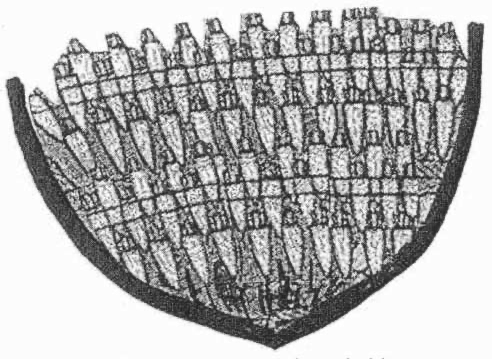
\includegraphics[width=.8\textwidth]{amphora_stowage_aboard_ship.png}
    \end{center}
    \caption{The egg-like shape enabled amphoras to interlock and minimize the waste of space on a ship.
    Source: \cite{twede2002commercial}.}
  \end{figure}

  Amphoras' various shapes and markings - which changed by time, region, producer, contents, and brand
  identity - were used to identify the package status and the different products inside \cite{twede2002commercial}.

  \begin{figure}[ht]
    \begin{center}
      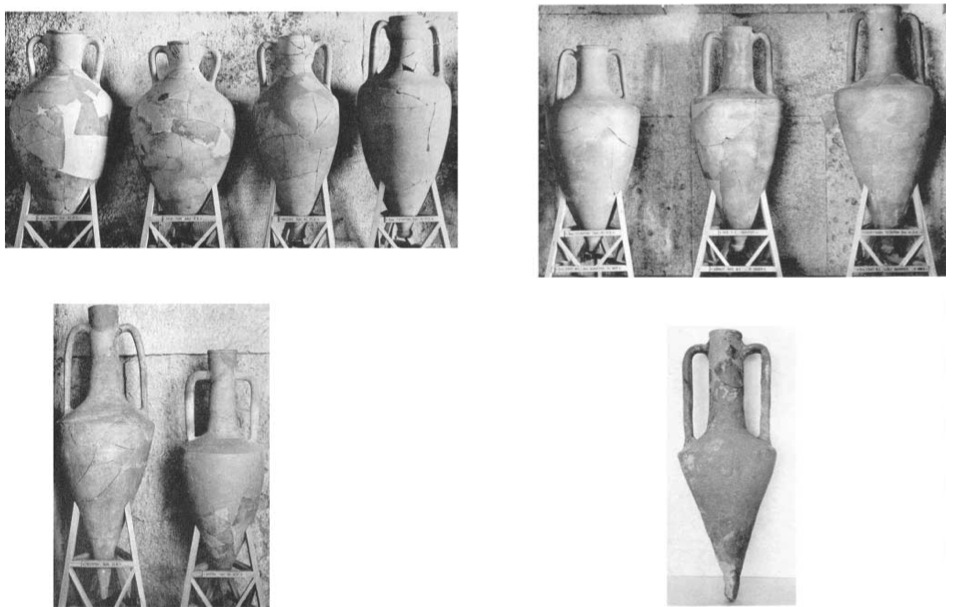
\includegraphics[width=.8\textwidth]{amphora_various_shape.png}
    \end{center}
    \caption{Amphoras have various shapes. Source: \cite{twede2002commercial}.}
  \end{figure}

  Amphoras have great significance in archaeology. They can be used as evidence for the trade patterns throughout
  the Mediterranean \cite{twede2002commercial}. As they were usually discarded at the destination of a trade and have been
  found in shipwrecks, archaeologists have been using them to recreate the transit routes \cite{twede2002commercial}.
  Furthermore, researchers have been able to classify different amphoras, which also helps to date ruins and shipwrecks
  \cite{twede2002commercial}.

  \subsubsection{Computer Vision for Underwater Object Detection}

  Computer vision is the science of perceiving and understanding the world through images and videos \cite{elgendy2020deep}.
  There have been multiple exciting applications of computer vision, including image classification \cite{rawat2017deep},
  object detection and localization \cite{zhao2019object,liu2020deep}, art generation (neural style transfer)
  \cite{jing2019neural}, image creation with Generative Artificial Networks (GAN) \cite{goodfellow2014generative},
  face recognition \cite{parkhi2015deep}, action and activity recognition \cite{poppe2010survey}, human pose estimation
  \cite{toshev2014deeppose}, and image recommendation system \cite{niu2018neural}.

  However, there is still limited research for the application of computer vision and machine learning in archaeology,
  especially underwater archaeology, compared to other domains \cite{maaten2007computer, qin2015underwater}.
  Computer vision, instead of visual inspection, could be used to automate the assessment and classification of artifacts
  \cite{maaten2007computer}.

  Underwater computer vision has proven to be challenging, largely due to: 1) the distortion and attenuation caused by
  light propagation in water, and 2) the unrestricted natural environment with the abundance of marine life and suspended
  particles \cite{qin2015underwater, rizzini2015investigation, lu2017underwater}.

  Despite the challenges, computer vision has lower cost \cite{rizzini2015investigation} compared to sonar imagery
  \cite{abu2019statistically} and laser scanning \cite{gordon1992use}. Plus, the abundance of visual data obtained through
  autonomous underwater vehicles (AUVs), unmanned underwater vehicles (UUVs) \cite{lu2017underwater}, and seafloor cabled
  observatories \cite{qin2015underwater} enables us to utilize deep learning.


  \subsection{Deep Learning}

  \subsubsection{Artifical Neural Networks (ANN)}
  \subsubsection{Convultional Neural Networks (CNN)}
  \subsubsection{Deep Learning vs. Traditional Computer Vision}

  \subsection{Object Detection}

  Define object detection and introduce the sliding CNN approach.

  \subsubsection{Fully Convolutional Networks (FCN)}

  \subsubsection{General Object Detection Framework Components}

  \paragraph{Region Proposals}
  \paragraph{Network Predictions}
  \paragraph{Non-Maximum Suppression (NMS)}
  \paragraph{Metrics}

  \subsubsection{Region-Based Convultional Neural Networks (R-CNN)}

  \paragraph{R-CNN}
  \paragraph{Faster R-CNN}
  \paragraph{Faster R-CNN}

  \subsubsection{Single Shot Detector (SSD)}
  \subsubsection{You Only Look Once (YOLO)}

  \paragraph{YOLO}
  \paragraph{YOLOv2}
  \paragraph{YOLOv3}
  \paragraph{YOLOv4}
  \paragraph{YOLOv5}

  % TODO: Remove Related Work?
  \section{Related Work}


  \section{Data and Methods}

  This is the technical core of the thesis. Here you lay out your how
  you answered your research question, you specify your design of
  experiments or simulations, point out difficulties that you
  encountered, etc.

  (target size: 5-10 pages)

  \subsection{Data}
  \subsection{Model}
  \subsection{Model Training}

  \section{Evaluation}

  This section discusses criteria that are used to evaluate the
  research results. Make sure your results can be used to published
  research results, i.e., to the already known state-of-the-art.

  (target size: 5-10 pages)

  \begin{table}[ht]
    \begin{center}
      \begin{tabular}{cl}
        \toprule
        Number & Description \\
        \midrule
        7 & A lucky number in Western culture \\
        8 & A lucky number in Chinese and other Asian cultures \\
        42 & Answer to the ultimate question of life, the universe, and everything \\
        404 & Not found \\
        \bottomrule
      \end{tabular}
      \caption{Useless insights I gained with no further meaning}
    \end{center}
  \end{table}

  \subsection{Visual Evaluation}
  \subsection{Metric Evaluation}

  \section{Conclusions}

  Summarize the main aspects and results of the research
  project. Provide an answer to the research questions stated earlier.

  (target size: 1/2 page)

  \section{Future Work}

  \newpage

  \printbibliography

\end{document}
